
%(BEGIN_QUESTION)
% Copyright 2015, Tony R. Kuphaldt, released under the Creative Commons Attribution License (v 1.0)
% This means you may do almost anything with this work of mine, so long as you give me proper credit

Something is wrong with this regulated DC power supply circuit.  The output is supposed to be +10.0 volts, but instead it measures only about 1 volt:

$$\includegraphics[width=15.5cm]{i03190x01.eps}$$

Using your digital multimeter, you measure 10.0 volts between test points TP5 (red test lead) and TP4 (black test lead).  From this information, identify two possible faults (either one of which could account for the problem and all measured values in this circuit), and also identify two circuit elements that could not possibly be to blame (i.e. two things that you know {\it must} be functioning properly, no matter what else may be faulted) other than the 120 volt AC power source, on/off switch, and fuse.  The circuit elements you identify as either possibly faulted or properly functioning can be wires, traces, and connections as well as components.  Be as specific as you can in your answers, identifying both the circuit element and the type of fault.

\begin{itemize}
\goodbreak
\item{} Circuit elements that are possibly faulted
\item{1.}
\item{2.} 
\end{itemize}

\begin{itemize}
\goodbreak
\item{} Circuit elements that must be functioning properly
\item{1.} 
\item{2.} 
\end{itemize}

\vfil 

\underbar{file i03190}
\eject
%(END_QUESTION)





%(BEGIN_ANSWER)

This is a graded question -- no answers or hints given!

%(END_ANSWER)





%(BEGIN_NOTES)

The fact we measure exactly 10.0 volts across the zener diode tells us everything between that zener and the AC power supply is functioning properly, and that therefore the problem must lie with either the opamp, the transistor, or some other component to the right.

Specifically, we are looking for a fault which would explain a total lack of voltage at the output terminals of the circuit, despite having precisely the right amount of reference voltage at the opamp for it to perform its voltage-regulation function.

\vskip 10pt

Note: the following answers are not exhaustive.  There may be more circuit elements possibly at fault and more circuit elements known to be functioning properly!

\begin{itemize}
\goodbreak
\item{} Circuit elements that are possibly faulted
\item{1.} Transistor $Q_1$ failed open (collector-to-emitter)
\item{2.} Broken wire/trace between opamp inverting input terminal and power supply ``+'' output terminal
\item{3.} Broken wire/trace between opamp non-inverting input terminal and zener diode
\item{4.} Broken wire/trace between opamp output terminal and transistor base terminal
\item{5.} Opamp $U_1$ output failed ``low''
\end{itemize}

\begin{itemize}
\goodbreak
\item{} Circuit elements that must be functioning properly (besides 120 volt AC source, switch, and fuse)
\item{1.} Transformer
\item{2.} Rectifying diodes
\item{3.} Zener diode
\item{4.} Resistor $R_1$
\end{itemize}

%INDEX% Troubleshooting review: electric circuits

%(END_NOTES)


